\documentclass[11pt]{article}
\usepackage[margin=1in,a4paper]{geometry}
\usepackage{setspace}
\usepackage{fancyhdr}
\usepackage{indentfirst}
\usepackage{graphicx}
\usepackage{amsmath, amssymb}
\usepackage[hidelinks]{hyperref}
\usepackage{bookmark}
\usepackage{helvet} % Helvetica font (closest to Arial in LaTeX)
\usepackage{titlesec}
\usepackage{tikz}
\usepackage[natbibapa]{apacite}
\usepackage{enumerate}
\usepackage[font=it]{caption}
\usepackage[justification=raggedright,singlelinecheck=false]{caption}
\captionsetup[table]{justification=raggedright, singlelinecheck=false}
\usepackage{booktabs}
\usepackage{float}
\graphicspath{{images/}} 

% Set default font to Helvetica (Arial equivalent)
\renewcommand{\familydefault}{\sfdefault}

\pagestyle{fancy}
\fancyhf{}
\fancyhead[L]{\uppercase{forecasting the price of refined sugar}}
\fancyhead[R]{\thepage}

\author{Leinnarf} 
\begin{document} %-----------------------+ START +-----------------------

\onehalfspacing

\begin{titlepage}
    \begin{center}

        \begin{center}
            \begin{minipage}{0.2\textwidth}
                
\includegraphics[width=.8\textwidth]{bulsu_logo.png}
            \end{minipage}
            \begin{minipage}{0.5\textwidth}
                \centering
                \singlespacing
                \fontsize{10}{9}
                Republic of the Philippines\\
                \textbf{BULACAN STATE UNIVERSITY}\\
                City of Malolos, Bulacan\\
                \textbf{COLLEGE OF SCIENCE}\\
            \end{minipage}
            \begin{minipage}{0.2\textwidth}
                
\includegraphics[width=.8\textwidth]{cs_logo.png} 
            \end{minipage}
        \end{center}
        \vspace{1em}
        \hrule
        \vspace{2em}

        {\LARGE \bfseries \MakeUppercase{Forecasting the Price of  Refined Sugar in the Philippines using ARIMAX Model}\\}  
        \vspace{2em}

        { \bfseries
        Alanan, Lara Marie F. \quad 
        Baldeo, Kenneth Dlonyer R.\quad
        Hilario, Franniel Luigi C. \\
        Rivera, Racks Justin J.\quad
        Santos, Franz Lenard L.
        }
        \vspace{2em}

        {
            Submitted to: \\
            Dr. Valentine Blez L. Lampayan
            % Mathematics Department\\
            % College of Science\\
            % Bulacan State University
        }

        \vspace{2em}

        { 
            \small
            College of Science, Bachelor of Science in Mathematics
            With Specialization in Computer Science,
            Bulacan State University, Malolos, Bulacan
        }

        \vspace{3em}
   
        \begin{abstract}
            \onehalfspacing
            This study forecasts the monthly retail price of refined sugar in the Philippines using the ARIMAX model, with the inclusion of exogenous variables such as climate conditions, sugar production and withdrawals, exchange rate, and inflation. Using data from 2014 to 2024, the optimal model, ARIMAX(1,1,1), achieved a Mean Absolute Percentage Error (MAPE) of 5.21 percent, indicating high accuracy. The Short-term forecasts for early 2025 showed a MAPE of just 0.51 percent when compared to actual prices. The three-year forecast (2025-2027) suggests a stable price trend with minor fluctuations. Additionally, the results shows that statistical significance doesn't always align with predictive value. These results provide useful insights for policymakers, businesses, and the agricultural sector in planning and decision-making related to sugar pricing and supply management. 
        \end{abstract}
        
    \end{center}
\end{titlepage}

\newpage
\thispagestyle{empty}
\tableofcontents
\newpage

\section{Introduction}
\pagenumbering{arabic}
 Sugar is one of the most widely consumed commodities in the Philippines, essential to both household and commercial consumption. It is one of the key ingredients in manufacturing various goods such as pastries, beverages, and processed foods, ranging from small businesses to large scale industries. Thus, a change in sugar price may affect businesses, consumers, and the broader economy. Forecasting sugar price is essential for informed decision-making in agricultural planning, trade, and policy formulation. 

According to \citet{tabuco-2023}, the sugar industry is vital to the Philippine economy, employing more than 1.5 million people and making up to around 2 percent of the country’s gross domestic product (GDP). The sugarcane crop year in the Philippines generally runs from September up to August of the following year, harvesting typically occurs during the drier months. Majority of the sugarcane in the Philippines is grown in the Visayas and Mindanao regions, particularly in the province of Negros Occidental, Isabela, and Cagayan. Western Visayas produced about 13.2 million tons of sugarcane or about 56 percent of the total production in 2023. Thus, hailing the Negros Occidental as the “Sugar Bowl of the Philippines”, it allocates about 208,000 hectares of land for planting and harvesting sugarcane used for raw sugar production \citep{balita-2024A}.   

\indent In the Philippine market, sugar is typically classified into refined, washed, and 
brown. Of these, refined sugar is most widely used, especially in food processing and household consumption.  The dominant preference for refined sugar is supported by findings that processed foods account for 64 percent to 75 percent of total sugar intake among Filipino children and adolescents \citep{amarra-2024}. The price of refined sugar in the Philippines has exhibited a significant upward trend. Based on the historical data from the Sugar Regulatory Administration, the average price per kilogram rose from Php.55.66 in the 2015-2016 crop year to Php.96.20 in 2023-2024. This increase can be attributed to various factors such as climate-related disruptions, supply-demand imbalances, and rising global sugar prices. 

\indent According to \citet{sevilla-2021}, the slow decline in sugarcane area and low farm productivity, particularly in areas outside Negros Island is one of the factor for sugar production, Climate variability such as drought, too much rain or extreme weather event like typhoons have an adverse effect on production. For instance, super typhoon Odette in 2021 caused damage worth Php.1.5 billion to the sugarcane sector in Negros, negatively affecting the 2021-2022 crop year \citep{talavera-2022}. 

\indent Due to local production shortages during the 2022-2023 period, the Philippines imported around 730,400 metric tons of refined sugar, more than 200 percent in the previous period. The importation was imposed to meet the domestic demand at a time of low production output \citep{balita-2024B}. However, imports exposed the market to international price volatility. Since global sugar prices influence import cost, increases in the global sugar price index can directly raise local market prices \citep{vesper-2024}

\indent This study aims to forecast the price of refined sugar in the Philippines using a mathematical modeling approach that includes external factors. While including multiple predictors or external variables may improve forecast accuracy, it also adds computational complexity. Thus, this research aims to find a balance between model precision and interpretability in order to offer valuable insights for stakeholders in agriculture, industry, and government policy. 

\subsection{Related Studies}

\indent There are various studies about the use of the Autoregressive Integrated Moving Average (ARIMA) model and the Autoregressive Integrated Moving Average with Exogenous variable (ARIMAX) model in forecasting the price of basic commodities such as rice, cooking oil, and crop yield. A study by \citet{gopinath-2019} about the production of sugarcane forecasting, compares the ARIMA and ARIMAX model, and concludes that the ARIMAX model gives greater accuracy. Another study by \citet{pushpa} also dealt with the sugarcane yield forecasting and comparing the performance of ARIMA and ARIMAX model. The study shows that ARIMAX model performed well with lower error metrics than ARIMA in all time regimes. \citet{CookingOil}, provides a study about the performance of ARIMAX model on cooking oil price data in Indonesia. They compare the ARIMA and ARIMAX model  on its performance on forecasting the cooking oil price in Indonesia, the results shows the mean average percentage error of ARIMA and ARIMAX models, giving 17.69 percent and 17.31 percent respectively.  It appears that the ARIMAX model indeed performed better than the ARIMA model; the inclusion of exogenous variables resulted in more accurate forecasting. 

\indent In the Philippines, there are few studies about forecasting the price of sugar, most of the studies are about forecasting the price of basic commodities, particularly rice. A study by \citet{SelectedCommodities}, uses ARIMA model to forecast the monthly price of selected agricultural commodities in the Philippines. They compared different ARIMA orders to find the best fit for the selected price of the commodities. \citet{Onion} , provides a 6-year forecast on the retail price of egg, rice, and onion using ARIMA and Seasonal ARIMA (SARIMA) models. A study from \citet{Palay} uses the ARIMA model to forecast the production of palay and retail price of rice in the Philippines. The results suggest that ARIMA(4,1,1) was the best fit for the palay production, and ARIMA(1,1,1) for the retail price of rice. The forecasted retail price of rice continues to increase. 


\subsection{Statement of the Problem}
The price of refined sugar is influenced by various factors such as climate conditions, sugar production, government policies, and global market trends. Changes in sugar prices have a direct impact on Filipino households, food manufacturers, and businesses that rely on sugar as a primary ingredient. Despite its economic and social significance, there is limited research on accurately forecasting sugar prices using mathematical models that incorporate both historical price data and external variables to forecast future price movements.

This study aims to develop a forecasting model for the prices of refined sugar in the Philippines using the AutoRegressive Integrated Moving Average with Exogenous Variables (ARIMAX) model. The model integrates external factors such as production and withdrawals of refined sugar, global sugar prices, exchange rate from USD to PHP, temperature, total precipitation, and inflation to improve the reliability of forecast.  

The study seeks to address the following questions:

\begin{enumerate}
    \item Which external factors influence the price of refined sugar in the Philippines, and how strong is their impact?
    \item Can the ARIMAX model generate accurate predictions for future price of refined sugar?
    \item What are the projected price of refined sugar for the following:
    \begin{itemize}
        \item \textbf{Short term:} For the first quarter of 2025?
        \item \textbf{Long term:} For the year 2025 to 2027?
    \end{itemize}
\end{enumerate}

\subsection{Scope and Delimitations}
This study aims to forecast the monthly prices of refined sugar in the Philippines using a mathematical model, specifically, using the AutoRegressive Integrated Moving Average with Exogenous Variables (ARIMAX) model. The exogenous variables in the study are the factors that affect the price of refined sugar such as climate conditions, sugar production, global prices of sugar, Philippine peso exchange rate, inflation rate, and  withdrawals of refined sugar. Since the Negros Region hold 56 percent of the total sugar production in the Philippines, the climate data will be taken from this region. The data includes the monthly temperature and total precipitation. Climate data from other plantations/production will not be included in the study. The dataset used for this study covers the period from 2014 to 2024, using monthly time series data. 

This study excludes the importation data due to difficulties in accessing consistent monthly import figures. Import data are often reported on an annual basis, making it difficult to fit on a monthly interval for time series.  Additionally, the Philippines doesn’t import sugar regularly and only imports when necessary to meet domestic demand. As a replacement, the researcher will use monthly withdrawal data because it represents the demand for the sugar. It is assumed that the volume of imported refined sugar can be indirectly inferred as the difference between the sugar withdrawn and locally produced refined sugar, allowing the model to account for the shortfalls in supply without explicitly including importation as a variable.

The forecasting will be exclusively to the refined sugar, washed and brown sugar as well as the other byproduct of sugarcane like molasses are excluded in the study. Prices of products that rely on sugar are excluded in the study, this includes beverages, pastries, and other food products. These limitations are employed to narrow down the scope of the study. The exogenous variables are chosen based on their relevance, availability, and measurable impact on prices of refined sugar. Adding more variables may result in more accurate forecasting but with the cost of computational complexity and harder accessibility to the data. 



\subsection{Significance of the Study}
The study aims to forecast the prices of refined sugar in the Philippines. The findings in the study are essential as they would benefit the society affected by the sugar price changes in making decisions for the future. 


\noindent The following are the institutions that would benefit from this study:

\begin{itemize}
    \item \textbf{Government Agencies}\\
    The findings could determine the Philippines’ current state of sugar reserves and be used by the Sugar Regulatory Administration of the Philippines (SRA). The administrator and CEO of SRA can effectively make decisions regarding it including effectively importing and exporting sugar based on the supply and demand for the best price and quantity and for emergency shortages due to calamities and such.
    \item \textbf{Filipino Community}\\
	As they are particularly affected by these prices, they will benefit from making better financial decisions regarding their purchases of related goods. These goods include pastries such as bread and condiments like caramel and syrup that are utilized by various businesses and consumers.

    \item \textbf{Businesses}\\
    As the biggest consumer of sugar, it would help them create better decisions in proper inventory and management of sugar to build and maintain their businesses. They could make necessary adjustments for prices of pastries and beverages utilizing sugar that the businesses and tycoons are selling.

    \item \textbf{Researchers/Scholars}\\
	It would be significant for researchers as this is one of the economic indicators for the Philippines in terms of wealth or purchasing power of a country. They could also create further studies regarding sugar and price predictions referencing this study.

    \item \textbf{Agricultural Sector}\\
	The executives would be equipped to make better decisions for effective inventory and management of sugar reserves throughout the Philippines. It could help the SRA and the Philippine Statistics Authority for proper pricing of sugar and sufficient inventory in different regions throughout the Philippines. The study could create more opportunities and options for farmers, increasing better livelihoods.
\end{itemize}

\subsection{Preliminaries}
In this section, the concepts used in the modeling process were discussed in order understand the modeling process.  
\begin{enumerate}[I. ]
    \item \textbf{Time Series Analysis}\\
    A time series is a sequence of data points recorded or measured at successive points in time, usually at uniform intervals. Time series analysis involves methods for analyzing such data to extract meaningful statistics and characteristics, identify patterns (like trend and seasonality), and make forecasts. It is formally defined as a set of observations $\{y_{t}\}$ where each observations $y_{t}$ is associated with a specific time point $t$. These observations are typically ordered chronologically and recorded in various frequency (daily, monthly, quarterly, yearly) \citep{boxjenkins}.
                
    \item \textbf{ARIMAX model}\\
    The AutoRegressive Integrated Moving Average with Exogenous Variables (ARIMAX) model is an extension of the ARIMA model that incorporates external (exogenous) variables to improve the forecasting accuracy. To understand ARIMAX, it is essential to first understand the AutoRegressive Integrated Moving Average (ARIMA) model, it is a time series model that combines three components: 

    \begin{itemize}
        \item \textbf{AR (AutoRegressive)} - uses the dependency between an observation and a number of lagged observations. The value of the current observation is affected by the previous observations. 
        \item  \textbf{I (Integrated) }- involves differencing the data to make it stationary.
        \item  \textbf{MA (Moving Average)} - models the dependency between an observation and a residual error from a moving average model applied to lagged observations. It captures the errors from previous observations and how it affects the current observation. 
    \end{itemize}
    The ARIMAX model adds an exogenous term, allowing it to account for external variables that may impact the forecasted series. This makes ARIMAX particularly useful in scenarios where the behavior of a time series is partially explained by other time-dependent variables. 


    \textbf{Mathematical Formulation}

    \citet{boxjenkins} ARIMA forecasts are based on past values of the variable being forecast. ARIMA model requires a minimum sample size of about 35-40 time series observations and must be stationary time series data. A stationary time series has mean and variance constant over time. The general functional of ARIMA($p,d,q$) model is:
    
    $$
        \hat{Y_{t}} = c + \phi_{1}Y_{t-1} + \phi_{2}Y_{t-2} + ... + \phi_{p}Y_{t-p} + \theta_{1}e_{t-1} + \theta_{2}e_{t-2} + ... + \theta_{q}e_{t-q}  
    $$
    or 
    $$
        Y_{t} = c + \sum_{i=1}^{p} \phi_{i}Y_{t - 1} + \sum_{j = 1}^{q} \theta_{j} e_{t -j} + e _{t}    
    $$
    
    Where, $Y_{t}$ is target variable at time $t$, $\phi, \theta$ are the coefficient  of AR($p$) and MA($q$) respectively,$e _{t}$ is the error at time $t$, and $c$ constant or the intercept. 

    ARIMA(1,1,1) is written as $Y_{t}= c + Y_{t -1} + \phi_{1}(Y_{t - 1} - Y_{t - 2}) - \theta_{1}e_{t - 1}$

    The general formula for the ARIMAX model, combines the ARIMA structure with exogenous variables 
    $$
        Y_{t} = c + \sum_{i=1}^{p}\phi_{i}Y_{t - i} + \sum_{j=1}^{q} \theta_{j}e_{t - j} + \sum_{k = 1}^{K} \beta_{k}X_{k,t} + e_{t}    
    $$

    As an extension of the ARIMA model, all of its component is present in the ARIMAX model with the inclusion of $X_{t}$ which represent the exogenous variable at time $t$, $\beta$ as the coefficient of the exogenous variable, and $K$ as the number of exogenous variables. 



    \item \textbf{Augmented Dickey-Fuller test for Stationarity}\\
    The Augmented Dickey-Fuller (ADF) test is a statistical test used to determine whether a time series is stationary or contains a unit root, which would indicate non-stationarity. In the ADF test, the null hypothesis ($H_{0}$) posits the presence of a unit root in the time series data, which implies non-stationarity. A unit root is a characteristic that causes the statistical properties of the series such as mean and variance to change over time. To determine whether a time series is stationary, the ADF test examines the p-value associated with the test statistic. If the p-value is less than the conventional significance level of 0.05, the null hypothesis is rejected, indicating that the unit root is not present and the series is stationary. When a series is not initially stationary, differencing is often applied. This transformation can eliminate the unit root by stabilizing the mean and variance of the data, thereby converting the series into a stationary one \citep{ADF}.

    \item \textbf{Autocorrelation function and Partial autocorrelation function}\\
    The Autocorrelation Function (ACF) and Partial Autocorrelation Function (PACF) are key tools in time series analysis, especially for identifying the appropriate order of ARIMA models. The ACF measures the correlation between a time series and its lagged values, capturing both direct and indirect influences from past observations. In contrast, the PACF measures the correlation between the series and its lagged values after removing the effects of shorter lags, isolating the direct impact of each lag. These functions are used to determine the parameters of the ARIMA model: the order of the autoregressive component (p) is identified using the PACF, while the order of the moving average component (q) is determined using the ACF. Specifically, if the PACF plot shows a sharp cutoff after lag p while the ACF tails off gradually, it suggests an AR(p) model. Conversely, if the ACF cuts off after lag q and the PACF tails off, it indicates an MA(q) model. When both ACF and PACF tail off, an ARMA(p, q) model may be appropriate \citep{acf}.

    \item \textbf{Ljung-Box Statistics Test}\\
    Ljung-Box Statistics Test is the statistical test that checks if autocorrelation exists in a time series \citep{ljung}. It is named by the statisticians Greta M. Ljung and George E.P. Box. It is defined by $H_{0}$: the model does not exhibit lack of fit, $H_{a}$: the model exhibits lack of fit, test statistic: Given a time series of length, the test statistic is defined as: 
    $$
        Q = n (n + 2) \sum_{k=1}^{m} \frac{\hat{r_{k}}^{2}}{n - k}  
    $$
    where $\hat{r_{k}}^{2}$ is the estimated autocorrelation of the series at lag $k$, and $m$ is the number of lags being tested, the significance level $\alpha$, and lastly the critical region where the Box-Ljung test rejects the null hypothesis (indicating that the model has significant lack of fit) if $Q > \chi^{2}_{1 -a,h}$, where $\chi^{2}_{1 - a,h}$ is the chi-square distribution table value with h degrees of freedom and significance level $\alpha$. Because the test is applied to residuals, the degrees of freedom must account for the estimated model parameters so that $h=m-p-q$, where $p$ and $a$ indicate the number of parameters from the ARMA ($p$, $q$) model fits the data. The Ljung-Box Statistics Test would be useful in our study by finding the autocorrelation in the time series data presented in forecasting the price of sugar in the Philippines. Autocorrelation is the mathematical representation of the degree of similarity between a given time series and a lagged version of itself over successive time intervals. The lagged version is the previous data that will be used in forecasting future values in the time series of the study. The autocorrelation validates the residuals used in the test and if the autocorrelation exists (it didn’t behave like white noise), the model might be inadequate and the forecast would be deemed unreliable. The test would prevent inadequacy, forecast errors, and inadequate predictions, and validate the usage of the ARIMAX model in forecasting the price of sugar in the Philippines.

    \item \textbf{Variance Inflation Factor (VIF)}\\
    The Variance Inflation Factor (VIF) is a statistical measure used to detect the severity of multicollinearity in a multiple regression model. Multicollinearity occurs when two or more predictor (independent) variables in a regression model are highly correlated, making it difficult to isolate the individual effect of each variable on the dependent variable \citep{vif1}.

    The VIF for a given predictor variable is defined as:
    $$
        VIF_{i} = \frac {1}{1 - R^{2}_{i}}   
    $$
    Where $R_{i}^{2}$ is the coefficient of determination when the $i-$th predictor is regressed against all the other predictors (variables). 

    A VIF value of 1 indicates no correlation with other variables (no multicollinearity). A VIF between 1 and 5 suggests moderate correlation, generally acceptable. A VIF above 5 or 10 is a sign of high multicollinearity, which may require correction \citep{vif2}.

    \item \textbf{Akaike Information Criterion (AIC)}\\
    According to \citet{zajic}, the AIC or Akaike Information Criterion is a number that can be used to determine the measure of model fit, thus which multiple models are most likely to be the best model for the given data set. Emphasizing that the AIC scores of other models are compared, and determine which model has the better quality. Furthermore, AIC works by assessing how well the model fits the training set and applying a penalty term for the model’s complexity. The result the study wants is the lowest possible AIC, indicating the best quality model. Additionally, Zajic notes that AIC uses a model’s maximum likelihood estimation (log-likelihood) as a measure of fit. In the formula $-2\ln(L)+2k$, log-likelihood, defined by $L$, measures how likely one is to see their observed data, given a model. The model with the maximum likelihood is the one that “fits” the data the best, hence, the better the quality of a model is.

    \item \textbf{Bayesian Information Criterion (BIC)}\\
    \citet{kumar} states that the Bayesian Information Criterion (BIC) is another model selection criterion that considers both model fit and complexity. Additionally, BIC is based on Bayesian principles and provides a stronger penalty for model complexity compared to AIC. Derived from the formula of AIC, the formula for BIC is $-2\log(L)+k\log(n)$. Furthermore, the term $\log (n)$ represents the logarithm of the sample size ($n$). This term in BIC introduces a stronger penalty for model complexity compared to AIC, as the penalty term scales with the sample size. Due to the higher penalty that BIC accounts for, it tends to create a bias toward simpler models compared to AIC, promoting a cheaper approach to model selection.

\end{enumerate}

\section{Methodology}
This study will employ a quantitative research design using time series analysis to forecast the price of refined sugar in the Philippines. The main forecasting technique to be used is the Autoregressive Integrated Moving Average with Exogenous Variables (ARIMAX) model. This model combines autoregressive and moving average components with exogenous variables that influence the target variable, i.e, the price of refined sugar.  

\subsection{Data}
The dataset used in this study consists of monthly time series data from September 2014 to August 2024, which corresponds to the crop year 2014-2015 to 2023-2024. All the variables were structured on a monthly interval to ensure consistency with the ARIMAX model. The variables include:

\textbf{Target Variable:}

\begin{itemize}
    \item Monthly retail \textbf{price of refined sugar} per kilogram in Metro Manila, collected from the Sugar Regulatory Administration (SRA). This serves as the variable to be forecasted
\end{itemize}
    
\textbf{Exogenous Variables:}

\begin{itemize}
    \item Climate data such as monthly \textbf{temperature} in Celsius and total \textbf{precipitation} in millimeter from Weather Underground. Focusing on the Negros Region, which accounts for 56 percent of national sugar production. These climate factors influence the sugarcane yield and harvest cycles.

    \item Refined sugar \textbf{production} and \textbf{withdrawals} in 50 kilograms-bag also from the Sugar Regulatory Administration (SRA).  Sugar production reflects the supply, while the withdrawals represent the demand.

    \item \textbf{Global sugar prices} (in USD) from Macrotrends. These prices reflect international market conditions that can affect the local pricing.

    \item \textbf{Exchange rate} (PHP to USD) from Bangko Sentral ng Pilipinas (BSP), included due to its impact on the cost of imported inputs and the competitiveness of domestic sugar in global markets. 

    \item \textbf{Inflation rates} are also collected from BSP to account for the general rise in price level which may influence the cost of refined sugar. 


\end{itemize}
All datasets are aligned to a monthly interval to maintain consistency and ensure model compatibility.  The entire dataset will be split into two subsets:
\begin{itemize}
    \item \textbf{Training Set:} 80 percent of the data will be used to fit and develop the ARIMAX model.
    \item \textbf{Testing Set:} 20 percent of the data will be used to evaluate the accuracy of the forecasted results from the training set. 
\end{itemize}

\subsection{Procedures}
The analytical procedure for the model development and validation is done in Python using various libraries such as \texttt{pandas, statsmodels, sklearn, pmdarima, matplotlib}, and it consists of the following stages: 

\begin{enumerate}
    \item \textbf{Data Preparation}\\
    Making sure all of the data are aligned in monthly intervals and handling the missing data points. The missing data points are filled using the \texttt{forward\_fill()} function from \texttt{pandas} library in Python. Then, split the dataset into training and testing sets. 
    \item \textbf{Stationarity Test}\\
    The Augmented Dickey-Fuller (ADF) test is conducted on each variable to test for stationarity, the \texttt{adfuller()} function from the \texttt{statsmodels} library in Python will be used to perform the test. If the variable is not stationary (p-value $>$ 0.05), perform differencing to eliminate the presence of trend or seasonality, if it is still stationary, differentiate it again until it achieves stationarity. This process was applied to the dependent variable and to exogenous variables.
    \item \textbf{Model Identification}\\
    Finding the appropriate order of ARIMAX($p,d,q$) parameters through the plot of Autocorrelation function (ACF) and Partial Autocorrelation Function (PACF). The AR components are determined using PACF plot, the lags with significant spikes are the possible order for the AR component. On the other hand, MA components are determined using ACF plot, the lags with significant spikes are the possible order for the MA component. The Integrated $I$ component is determined based on the order of differencing required to achieve stationarity. 
    \item \textbf{Model Estimation and Selection}\\
    All of the possible ARIMAX models are fitted using the training set and evaluated for accuracy with the test set. Each model is assessed based on mean absolute percentage error (MAPE) to measure the forecasting accuracy, Akaike information criterion (AIC) and Bayesian information criterion (BIC) to penalize model complexity.The best ARIMAX model is selected based on the lowest values of AIC, BIC, and MAPE. 
    \item \textbf{Model Diagnostics and Interpretation}\\
    The residuals of the selected model will be examined using the Ljung-Box test to ensure that the residuals resemble white noise. The coefficients of the variables are interpreted based on their significance (p-values). Variance inflation factor (VIF) may be calculated to assess multicollinearity among exogenous variables. 
    \item \textbf{Forecasting}\\
    Once the best-performing ARIMAX model was selected, it will be used to forecast the monthly retail price of refined sugar in the Philippines. For the forecasting of each exogenous variable, the ARIMA model will be used along with the \texttt{auto\_arima()} function from \texttt{pmdarima} library in Python to find the order of parameters. The forecasted are generated for the short-term(first quarter of 2025) and long-term period (from 2025 to 2027).
\end{enumerate}

The Flowchart shows the procedure for the modeling process:
\vspace{12pt}

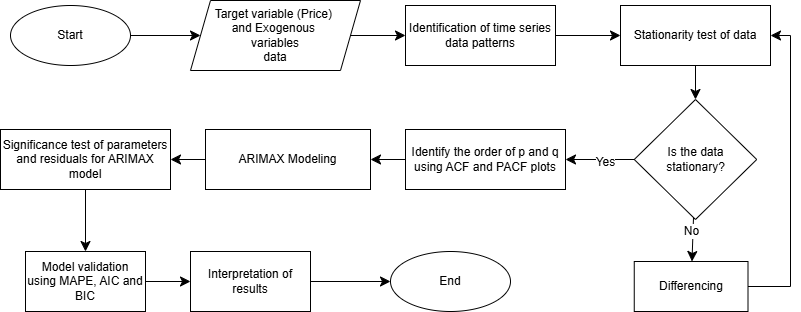
\includegraphics[width=\textwidth]{flowchart.png}

\subsection{Error Metrics}

The performance of the ARIMAX model is evaluated using the following error metrics:

\begin{itemize}
    \item \textbf{Mean Absolute Error (MAE)}: The average of the absolute differences between the predicted and actual values. It provides a measure of how close predictions are to the actual outcomes. 
    $$
        MAE = \frac{1}{n} \sum_{i=1}^{n} |y_{i} - \hat{y}_{i}|  
    $$

    \item \textbf{Mean Absolute Percentage Error (MAPE)}: The average of the absolute percentage errors between the predicted and actual values. It is useful for understanding the accuracy of the model in relative terms.

    $$
        MAPE = \frac{1}{n} \sum_{i=1}^{n} \left| \frac{y_{i} - \hat{y}_{i}}{y_{i}} \right| \times 100  
    $$

    \item \textbf{Root Mean Square Error (RMSE)}: The square root of the average of the squared differences between predicted and actual values. It gives more weight to larger errors and it is sensitive to outliers
    
    $$
        RMSE = \sqrt{\frac{1}{n} \sum_{i=1}^{n} (y_{i} - \hat{y}_{i})^{2}}  
    $$
\end{itemize}

Among these, MAPE is prioritized as the primary evaluation metric because of its interpretability in comparing the forecast accuracy. A MAPE value below 10 percent is commonly regarded as highly accurate, while values between 10 and 20 percent are considered good for practical forecasting purposes \citep{lewis}. MAE and RMSE were used as supplementary metrics to the scale and variability of the errors. 


\begin{table}[H]
    \caption{\textit{MAPE Forecast Accuracy Rating \citep{lewis}}}
    \label{lewis}
    \centering
    \begin{tabular}{lc}
        \toprule
        MAPE (\%) & Forecast Accuracy \\
        \midrule
        $< 10\%$ & Highly accurate forecast \\
        $10\%$ to $<20\%$ & Good forecast \\
        $20\%$ to $< 50\%$ & Reasonable forecast \\
        $\ge 50\%$ & Inaccurate forecast \\
        \bottomrule
    \end{tabular}
\end{table}

\section{Results and Discussion}

\subsection{Modeling Process}

Figure \ref{price_plot} shows the Price of Refined Sugar in the Philippines starting from September 2014 up to August 2024. The plot shows a significant increase in 2022 due to the typhoon Odette. An upward trend is evident in the plot, suggesting that the time series data is not stationary. 
\begin{figure}[h]
        \caption{Monthly time series plot of the price of refined sugar in the Philippines}
        \centering
        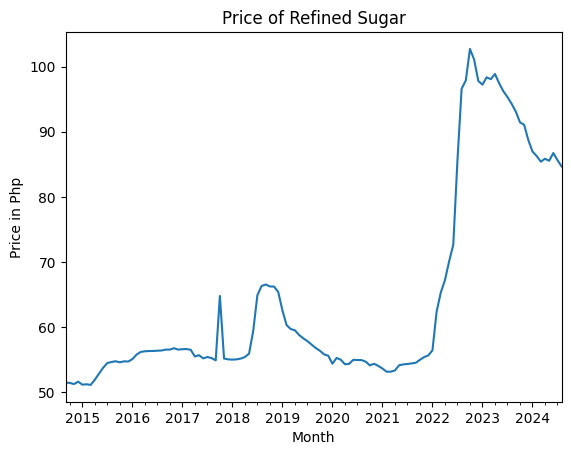
\includegraphics[width=0.75\textwidth, height = 3in]{Price_plot.png}
        \label{price_plot}
\end{figure}
    
Performing the Augmented Dicky-Fuller test on the data shows a P-value of 0.664, confirming that the time series data is not stationary. Performing first-order differencing stabilizes the data and eliminates the trend, resulting in p-value of 0.0000057 making the data stationary. Thus, the order for the parameter $d = 1$. 

\begin{figure}[h]
    \caption{Differenced time series plot of the price of refined sugar}
    \centering
    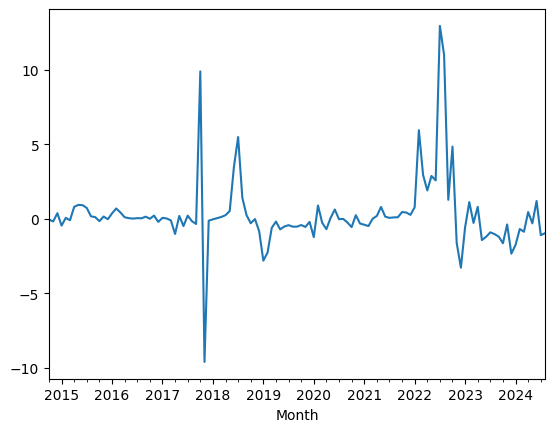
\includegraphics[width = 0.75\textwidth,height = 3in]{differenced.png}
    \label{diff}
\end{figure}

\begin{figure}[h]
    \caption{Train-test split}
    \centering
    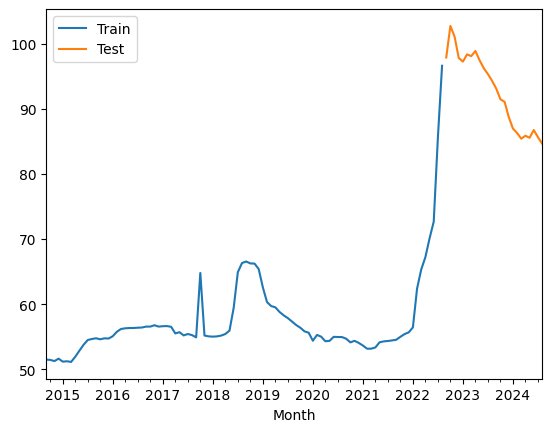
\includegraphics[width = 0.75\textwidth,height = 3in]{split.png}
    \label{split}
\end{figure}

Figure \ref{split} split the target variable (price of refined sugar) along with the exogenous variables  into a training set and test set. Data from September 2014 to August 2022 are in the training set, while the data from September 2022 to August 2024 are in the test set that will be used for evaluating the model. 

The plot of the Autocorrelation function (ACF) and the Partial Autocorrelation function (PACF) of the differenced data is shown in figure \ref{acf_pacf}. It is used to determine the order of $p$ and $q$ parameter for the AR and MA component. 

\begin{figure}[h]
    \caption{ACF and PACF plot of the train set}
    \centering
    \begin{minipage}{0.48\textwidth}
        \centering
        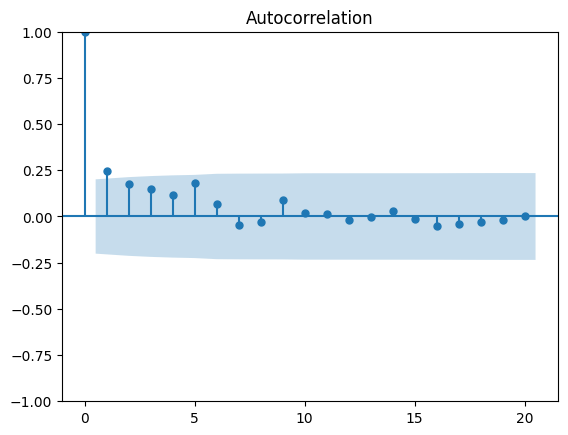
\includegraphics[width=\linewidth]{acf.png}
    \end{minipage}
    \hfill
    \begin{minipage}{0.48\textwidth}
        \centering
        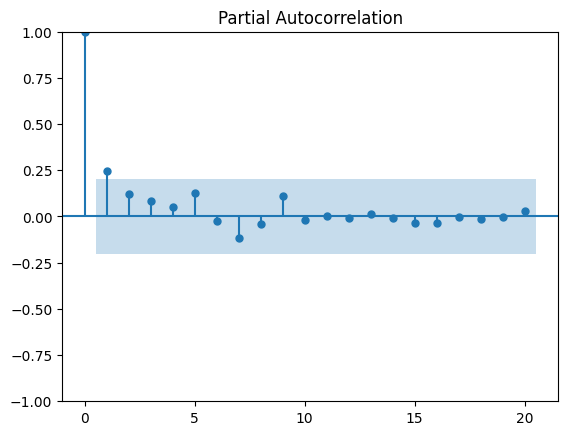
\includegraphics[width=\linewidth]{pacf.png}
    \end{minipage}
    \label{acf_pacf}
\end{figure}

Figure \ref{acf_pacf} suggest that the order of $p = [1]$ and $q = [1]$. Thus ARIMAX(1,1,1) was the only possible model. The performance of the model is shown in the table \ref{arimax111}, and the forecasted plot is in Figure  \ref{traintest} 

\begin{table}[H]
    \caption{\textit{Performance Metrics of ARIMAX(1,1,1) Model}}
    \label{arimax111}
    \centering
    \begin{tabular}{lccccc}
        \toprule
        Model & MAE & MAPE & RMSE & AIC & BIC \\
        \midrule
        ARIMAX(1,1,1) & 4.58 & 5.21\% & 6.25 & 443.81 & 469.35 \\
        \bottomrule
    \end{tabular}
\end{table}

The forecasted result shows a highly accurate forecast, with a mean average percentage error of $5.21\%$ 

\begin{figure}[h]
    \caption{Forecasted result of ARIMAX(1,1,1) model on the train set}
    \label{traintest}
    \centering
    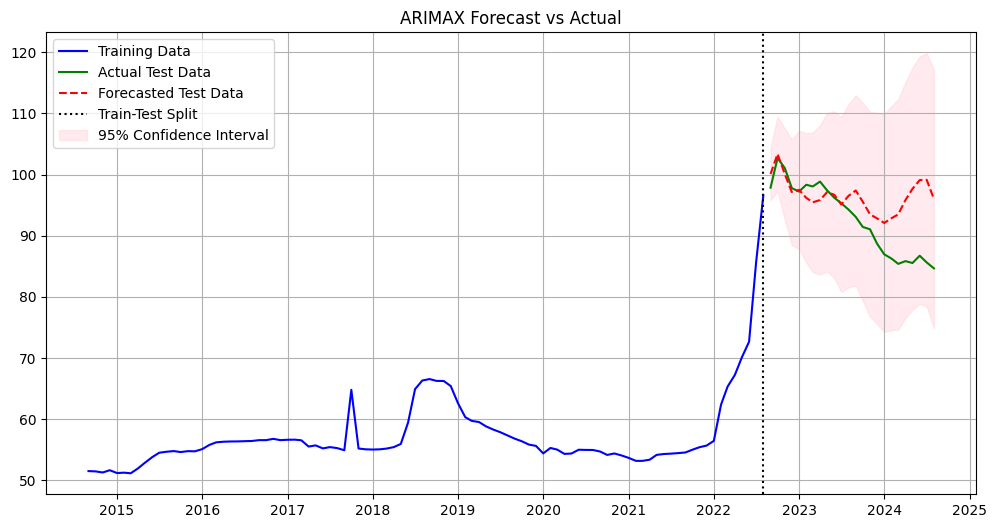
\includegraphics[width = \textwidth]{train_test_forecast.png}
    The numerical values are presented in \textbf{\ref{test_pred_table}}
\end{figure}


\newpage

The residuals of the model is shown in figure \ref{resid}, and its the ACF and PACF plot in figure \ref{resid_acf_pacf}. The plot of the ACF shows no autocorrelation in the residuals, which is a good sign that the residuals behave like white noise. 


\begin{figure}[h]
    \caption{Plot of the residuals of the model}
    \centering
    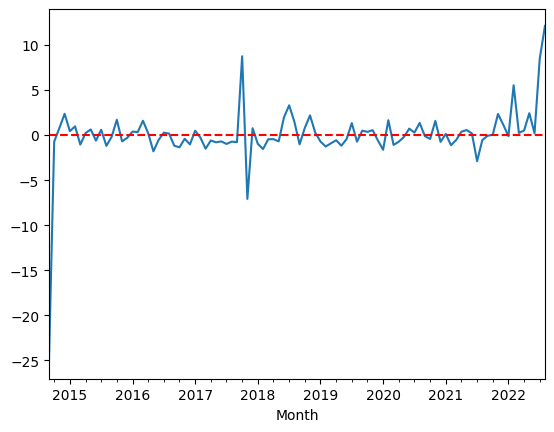
\includegraphics[width = 0.75\textwidth,height = 3in]{resid.png}
    \label{resid}
\end{figure}

\begin{figure}[h]
    \caption{ACF and PACF plot of the residuals of the model}
    \centering
    \begin{minipage}{0.48\textwidth}
        \centering
        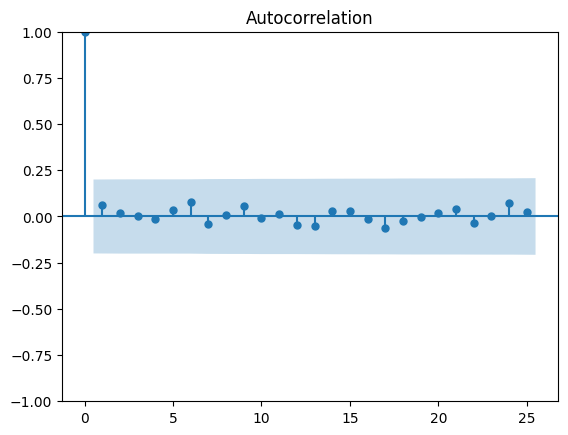
\includegraphics[width=\linewidth]{resid_acf.png}
    \end{minipage}
    \hfill
    \begin{minipage}{0.48\textwidth}
        \centering
        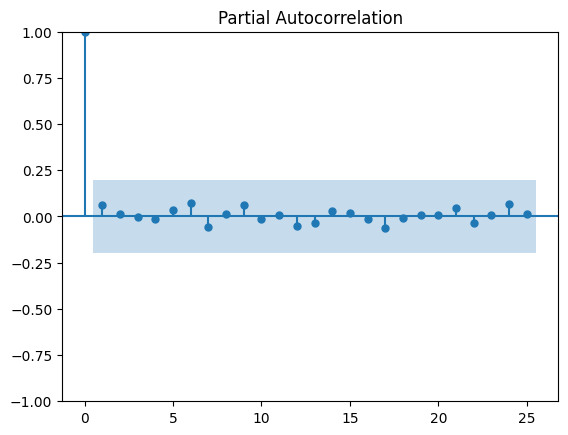
\includegraphics[width=\linewidth]{resid_pacf.png}
    \end{minipage}
    \label{resid_acf_pacf}
\end{figure}

Ljung-Box test was performed in the model's residuals to further justify that the residuals resemble white noise and no autocorrelation exist. The result of the test is shown in the table \ref{ljungbox}, the p-value for all 12 lags are higher than 0.05. Hence, the residuals shows no autocorrelation and it resembles white noise, increasing the validity of the model. 

\begin{table}[H]
    \caption{\textit{Ljung-Box Test Statistics for Residuals Autocorrelation}}
    \label{ljungbox}
    \centering
    \begin{tabular}{cc|cc}
        \toprule
        Lag  & p-value & Lag & p-value  \\
        \midrule
        1  & 0.524 &  7 & 0.985 \\
        2  & 0.805 &  8 & 0.994 \\
        3  & 0.933 &  9 & 0.995 \\
        4  & 0.979 & 10 & 0.998 \\
        5  & 0.990 & 11 & 0.999 \\
        6  & 0.977 & 12 & 0.999 \\
        \bottomrule
    \end{tabular}
\end{table}

Variance Inflation factor was used to determine if multicollinearity exists, using the \texttt{\\ variance\_inflation\_factor()} function from \texttt{statsmodels}in Python. The results in table \ref{vif} shows a low multicollinearity among the variables. 
\begin{table}[H]
    \caption{\textit{Variance Inflation Factor (VIF) of the Exogenous Variables}}
    \label{vif}
    \centering
    \begin{tabular}{lc}
        \toprule
        Variable & VIF  \\
        \midrule
      Production  &  2.99 \\
      Withdrawals  &  1.77 \\
      Global Price  &  1.44     \\ 
      Exchange Rate  &   2.53    \\ 
      Temperature  &   1.2    \\ 
      Precipitation  &   2.56   \\
      Inflation &   2.23    \\ 
        \bottomrule
    \end{tabular}
\end{table}

\begin{table}[H]
    \caption{\textit{ARIMAX(1,1,1) model Summary}}
    \label{signficance}
    \centering
    \begin{tabular}{lccr}
        \toprule
        Variable & Coefficient & P-value & Interpretation \\
        \midrule
        Production  & -2.006e-07 &  0.832  &  Not significant \\
        Withdrawals & 2.414e-07 &  0.811  &  Not significant  \\
       Global Price  & -10.4240   &  0.000  &  Highly significant \\ 
        Exchange Rate&  1.4639    &  0.000  &  Highly significant\\ 
        Temperature   &  0.2915    &  0.521  &  Not significant\\ 
        Precipitation &  0.0041    &  0.186  &  Somewhat significant \\
         Inflation &  0.8710    &  0.382  &  Not significant \\ 
        AR(1), MA(1)   &   ~0       & ~1.000  &  Not contributing to the model \\
        \bottomrule
    \end{tabular}
\end{table}

\newpage

\noindent The results in table \ref{signficance} shows that the following must be consider:

\begin{enumerate}
    \item \textbf{The coefficients for AR(1) and MA(1) are both zero and not contributing to the model. }
    
    Since the AR and MA component is not contributing a lot to the model, ARIMAX(0,1,0) might work. However, ARIMAX(0,1,0) shows a higher AIC and BIC than ARIMAX(1,1,1), thus the ARIMAX (1,1,1) is still the better model. The differencing might remove the autocorrelation or the exogenous variables explain most of the variation, leaving little autocorrelation structure for AR and MA to capture. 
    \begin{table}[H]
        \caption{\textit{Performance Metrics of ARIMAX(1,1,1) vs ARIMAX(0,1,0)}}
        \label{arimax010}
        \centering
        \begin{tabular}{lccccc}
            \toprule
            Model & MAE & MAPE & RMSE & AIC & BIC \\
            \midrule
            ARIMAX(1,1,1) & 4.58 & 5.21\% & 6.25 & 443.81 & 469.35 \\
            ARIMAX(0,1,0) & 4.58 & 5.21\% & 6.25 & 778.34 & 798.77 \\
            \bottomrule
        \end{tabular}
    \end{table}

    \item \textbf{Some of the variables are not significant based on their p-value, leaving Global Price and exchange rate with high significance.}

    Excluding the insignificant exogenous variable in the model and including only the significant variables (Global price and Exchange rate) performed worse than with all exogenous variables. Hence, keeping all the exogenous variables in the model despite its insignificance improved the forecasting performance. 

    \begin{table}[H]
        \caption{\textit{Performance Metrics of ARIMAX(1,1,1) with all exogenous variable vs only the significant variables}}
        \label{exog_significant}
        \centering
        \begin{tabular}{lccccc}
            \toprule
            ARIMAX(1,1,1) & MAE & MAPE & RMSE & AIC & BIC \\
            \midrule
            With all Exogenous variables & 4.58 & 5.21\% & 6.25 & 443.81 & 469.35 \\
            Only the significant variables & 17.32 & 18.51\% & 17.72 & 668.23 & 688.66 \\
            \bottomrule
        \end{tabular}
    \end{table}

    \item \textbf{The coefficient of the Global Price is negative, which is counterintuitive.}

    The negative coefficient of in Global price may suggest that the increase in global price decreases the local price. Normally, the global price act as a benchmark for the local price, an increase in global price may also increase the local price. The decision was made to exclude this variable in the model to preserve interpretability. The result in table \ref{noglobal}, shows minimal difference, but the model with no global price has slightly lower AIC and BIC score. 
    
       \begin{table}[H]
        \caption{\textit{Performance Metrics of ARIMAX(1,1,1) with global price vs no global price variable}}
        \label{noglobal}
        \centering
        \begin{tabular}{lccccc}
            \toprule
            ARIMAX(1,1,1) & MAE & MAPE & RMSE & AIC & BIC \\
            \midrule
            With global price & 4.58 & 5.21\% & 6.25 & 443.81 & 469.35 \\
            No global price  & 4.95 & 5.62\% & 6.60 & 442.03 & 465.02 \\
            \bottomrule
        \end{tabular}
    \end{table}
     Given that the model without the global price variable achieved comparable predictive performance while yielding lower AIC and BIC values, it was selected as the final model to prioritize interpretability.
\end{enumerate}

Hence, the final model was the ARIMAX(1,1,1) with all the exogenous variables except global price. Despite the statistical significance of other exogenous variables, the final model shows more accurate forecasting performance.  

\subsection{Forecasting}

The model for the forecasting of price of refined sugar in the Philippines is the ARIMAX(1,1,1) with all the exogenous variables except global price. The forecasting for each exogenous variable was done using the ARIMA model, see \textbf{\ref{exog_plot}} for the forecast plot. The \texttt{auto\_arima()} function in the \texttt{pmdarima} library in Python, was used to find the optimal order for each exogenous variable. The range of the forecast is from September 2024 up to August 2027. 

\begin{figure}[H]
    \caption{Forecasting the Price of Refined sugar for 2025 to 2027}
    \label{forecast}
    \centering
    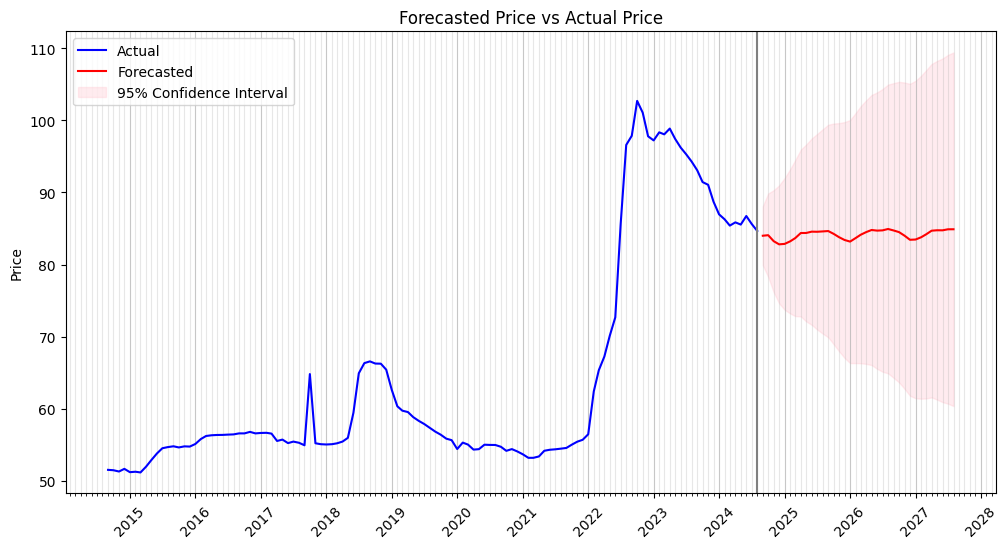
\includegraphics[width = 0.88\textwidth]{forecasted_plot.png}
    
    Confidence interval shows that the actual price lie within that range. The numerical values are presented in  \textbf{\ref{forecast_table}}
\end{figure}

The 3-year forecast shows a relatively stable trend with mild fluctuations and a slight upward tendency over time. The model is 95 percent confident that the actual price will lie within the confidence interval. To further justify the result of the model, actual latest price retrieved from Department of Agriculture price monitoring will be used to evaluate the forecasted price, ranging from September 2024 up to March 2025. 

\begin{table}[H]
    \caption{\textit{Forecasted Price vs Latest Actual Price of refined sugar}}
    \label{super}
    \centering
    \begin{tabular}{lcc}
        \toprule
        Date & Actual Price & Forecasted Price  \\
        \midrule
        September 2024 & 84 &    83.99 \\
        October 2024   & 83.15 & 84.07  \\
        November 2024  & 83.13 & 83.23  \\
        December 2024  & 82.83 & 82.80  \\
        January 2025   & 83.65 & 82.86  \\
        February 2025  & 83.07 & 83.22  \\
        March 2025     & 83.14 & 83.67  \\
        April 2025     & 83.49 & 83.37  \\
        \bottomrule
    \end{tabular}
\end{table}

\begin{table}[H]
    \caption{\textit{Evaluation of the Forecasted price}}
    \label{eval}
    \centering
    \begin{tabular}{ccc}
        \toprule
         MAE & MAPE & RMSE \\
        \midrule
        0.43 & 0.51\% & 0.56 \\
        \bottomrule
    \end{tabular}
\end{table}
The Forecasted price and the actual price shows a mean average percentage error of 0.51 percent, mean average error of 0.43, and root mean squared error of 0.56. For the longer-term, the forecasted price of refined sugar was ranging from 82.80 to 84.93 pesos per kilogram. It shows that the result of the forecast captured the actual price very well.

\section{Conclusion}

This study successfully developed an ARIMAX(1,1,1) model to forecast the monthly retail price of refined sugar in the Philippines by integrating key exogenous variables such as refined sugar production and withdrawals, the peso-to-dollar exchange rate, regional temperature and total precipitation in Negros region, and the national inflation rate. The model shows high predictive accuracy, with a Mean Absolute Percentage Error (MAPE) of 5.62 percent when evaluated with the test set,and 0.51 percent in short-term validation using data from late 2024 to early 2025, supported by a low Mean Absolute Error (MAE) of 0.43 and Root Mean Squared Error (RMSE) of 0.56. While the global price and exchange rate were statistically significant, the model's optimal performance was achieved when all exogenous variables (except global price) are included, demonstrating that statistical significance does not always align with predictive strength. Compared to other variants, the chosen ARIMAX(1,1,1) model captured underlying pattern most effectively and achieving the lowest AIC and BIC. The three-year forecast shows a relatively stable trend in the price of refined sugar, with mild fluctuations and a slight upward tendency over time, within a range of 82.80 to 84.93 pesos per kilogram. aWhile the forecast suggests stability, it is important to note that some degree of uncertainty is present, especially in longer-term projections as it is reflected in the widening of the confidence interval. Overall, the findings address the research objectives and offer valuable insights to support evidence-based policy and strategic planning for stakeholders across the sugar supply chain.
\subsection{Recommendations}
Although the findings of the study achieved good results, there are still areas in the study that need to be addressed, suggesting that there is room for improvements. The following are the recommended actions for future researchers to improve the study:

\begin{itemize}
    \item \textbf{Larger datasets}\\
    Expanding the dataset with a longer historical time frame in order to capture more underlying patterns in the dataset. This allows for better detection of long-term patterns and rare events in the dataset. 20-year historical data may suffice to capture the long-term patterns such as the trend and seasonality. Additionally, inclusion of additional exogenous variables such as transportation cost, energy prices, labor rates, and policy-related indicators that could influence the price of refined sugar. 

    \item \textbf{Different time series models}\\
    Exploring alternative time series models like seasonal ARIMAX (SARIMAX) model, or various Vector Autoregressive (VAR) such as VARMA (with Moving Average) and VARMAX (with Moving Average and exogenous regressors), may use to compare the ARIMAX performance. In addition, applying machine learning approaches like Random Forest, XGBoost, or LSTM could capture complex, nonlinear relationships among variables that traditional models might miss. 


    \item \textbf{Interpretation for the statistical significance}\\
    The interpretation of statistical significance of the external factors was not fully explored in the study. For instance, the negative coefficient in the global price of sugar seems counterintuitive, and the underlying cause of this was not investigated thoroughly in the paper. 
\end{itemize}

Future researchers may consider these recommendations to improve the study and provide a more comprehensive analysis of the price of refined sugar in the Philippines. Addressing these issues will enhance the robustness of the model and provide more accurate forecasts, benefiting stakeholders in the sugar industry.

\newpage
\section{References}
\renewcommand{\refname}{\vspace*{-2em}} 
\bibliographystyle{apacite}
\bibliography{tite.bib}

\newpage
\section{Appendix}


\renewcommand{\thesubsection}{A.\arabic{subsection}}

\subsection{Plot of the Exogenous variables with their forecasted values}
\label{exog_plot}

    \begin{figure}[H]
        \caption*{Monthly Production of Refined Sugar}
        \centering
        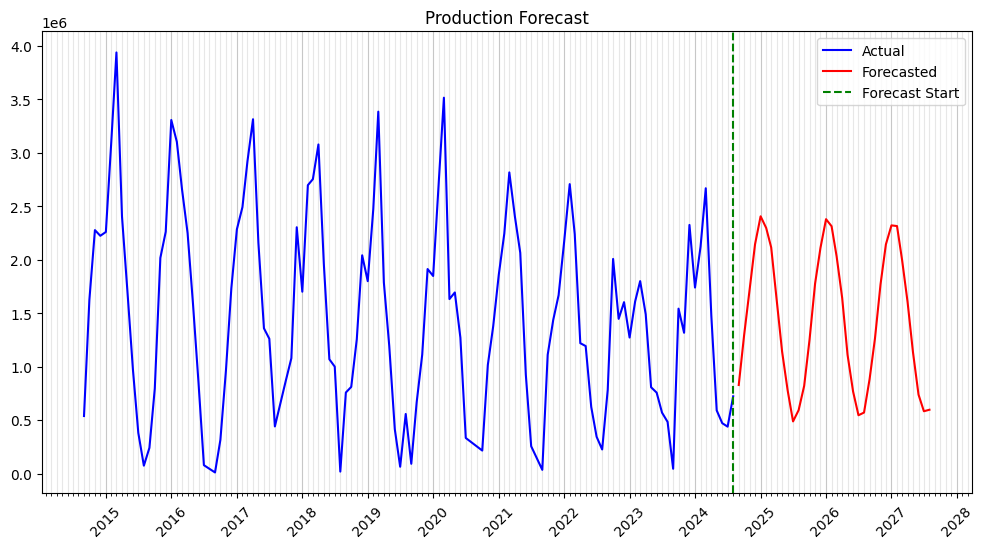
\includegraphics[width=0.75\textwidth]{production_plot.png}
        \label{production_plot}
    \end{figure}

    \begin{figure}[H]
        \caption*{Monthly Withdrawals of Refined Sugar }
        \centering
        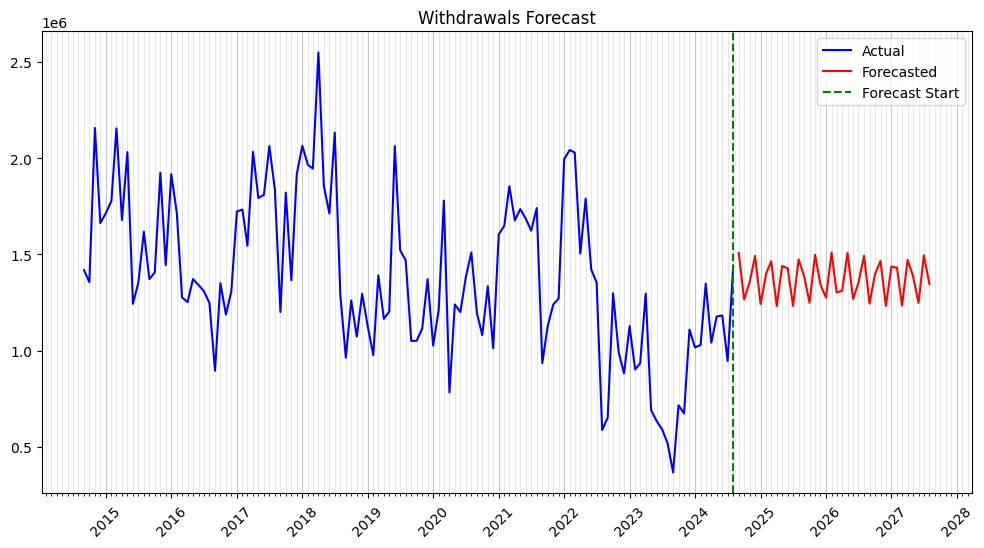
\includegraphics[width=0.75\textwidth]{withdrawals_plot.png}
        \label{withdrawals_plot}
    \end{figure}

    \begin{figure}[H]
        \caption*{Monthly Exchange Rate (PHP to USD)}
        \centering
        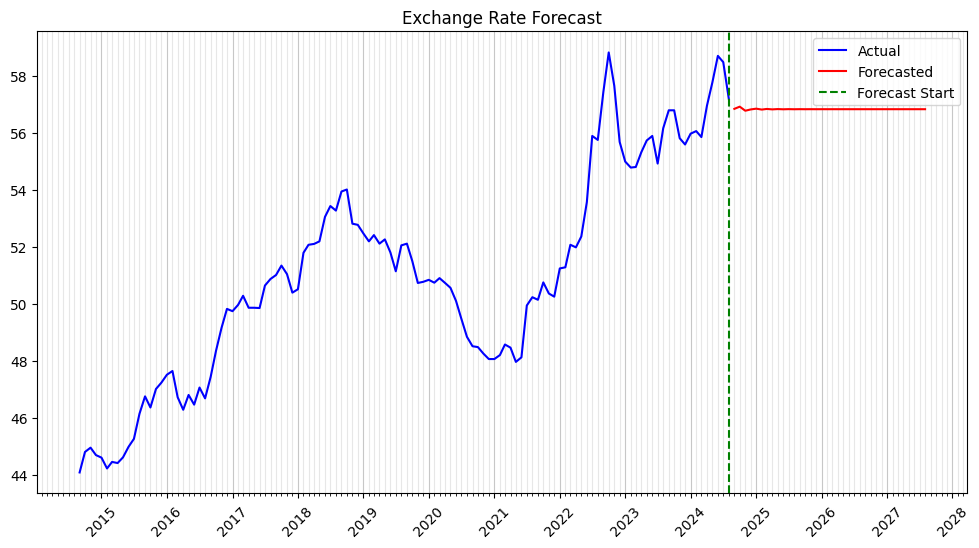
\includegraphics[width=0.75\textwidth]{exchange_rate_plot.png}
        \label{exchange_rate_plot}
    \end{figure}

    \begin{figure}[H]
        \caption*{Monthly Temperature in Negros Region }
        \centering
        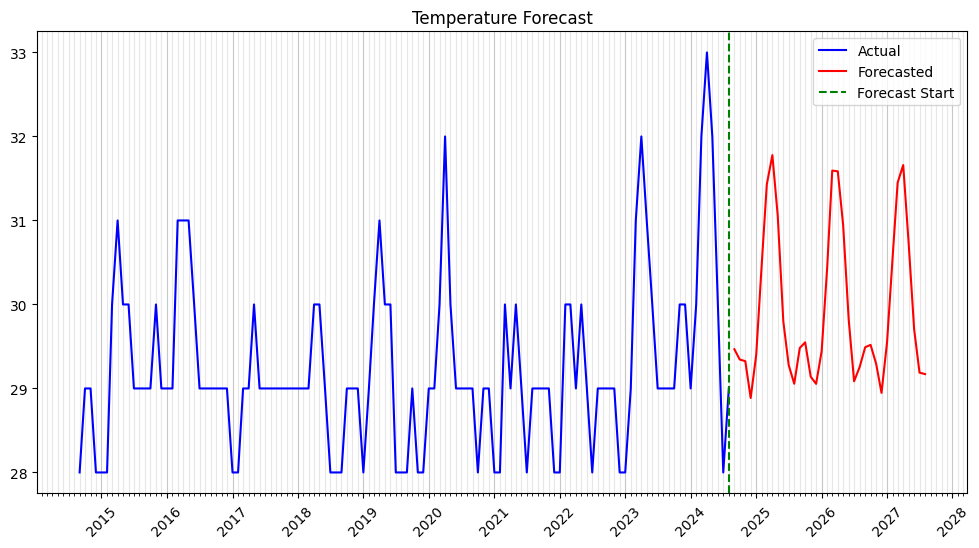
\includegraphics[width=0.75\textwidth]{temperature_plot.png}
        \label{temperature_plot}
    \end{figure}

    \begin{figure}[H]
        \caption*{Monthly Precipitation in Negros Region}
        \centering
        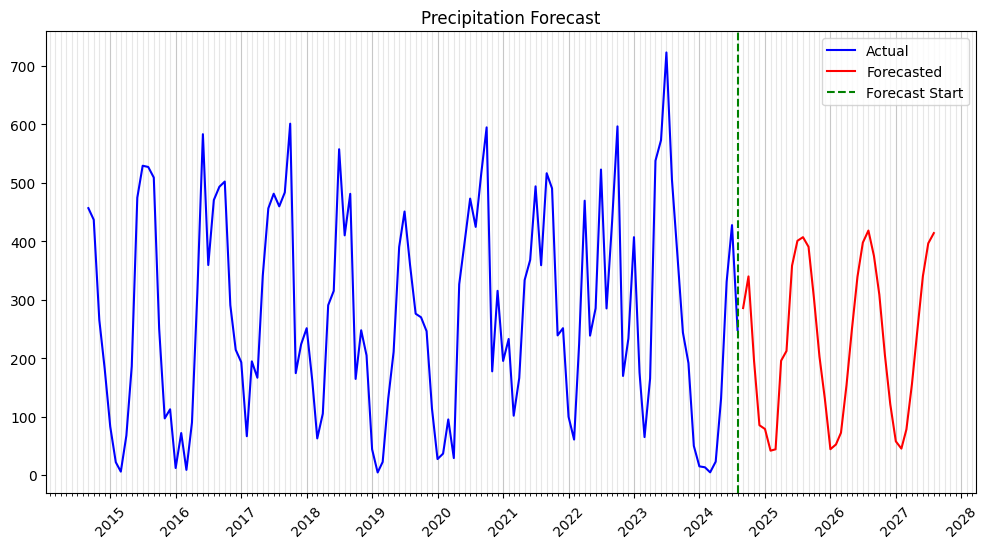
\includegraphics[width=0.75\textwidth]{precipitation_plot.png}
        \label{precipitation_plot}
    \end{figure}

    \begin{figure}[H]
        \caption*{Monthly Inflation Rate}
        \centering
        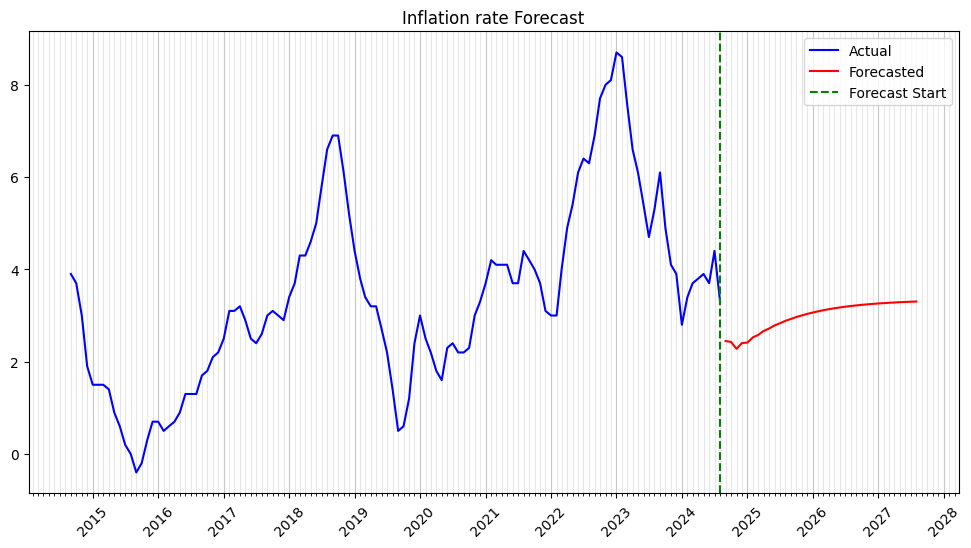
\includegraphics[width=0.75\textwidth]{inflation_plot.png}
        \label{inflation_plot}
    \end{figure}


\subsection{ARIMAX(1,1,1) results from train-test set}
\label{test_pred_table}

\begin{table}[H]
    \caption*{\textit{Model Forecast vs Test Set  with 95\% Confidence Interval (2022-2024)}}
    \centering
    \begin{tabular}{lcccccc}
        \toprule
        Date & Test & Pred & Difference & Lower CI & Upper CI \\
        \midrule
        2022-09-01 & 97.86 & 100.12 & -2.26 & 95.81 & 104.44 \\
        2022-10-01 & 102.70 & 103.45 & -0.75 & 97.34 & 109.55 \\
        2022-11-01 & 101.07 & 100.17 & 0.90 & 92.70 & 107.65 \\
        2022-12-01 & 97.79 & 97.20 & 0.59 & 88.57 & 105.84 \\
        2023-01-01 & 97.22 & 97.50 & -0.28 & 87.85 & 107.15 \\
        2023-02-01 & 98.34 & 96.32 & 2.02 & 85.75 & 106.89 \\
        2023-03-01 & 98.06 & 95.67 & 2.39 & 84.25 & 107.09 \\
        2023-04-01 & 98.86 & 96.52 & 2.34 & 84.32 & 108.73 \\
        2023-05-01 & 97.43 & 97.99 & -0.56 & 85.04 & 110.94 \\
        2023-06-01 & 96.22 & 97.51 & -1.29 & 83.86 & 111.16 \\
        2023-07-01 & 95.31 & 95.84 & -0.53 & 81.53 & 110.16 \\
        2023-08-01 & 94.28 & 97.27 & -2.99 & 82.31 & 112.22 \\
        2023-09-01 & 93.08 & 98.35 & -5.27 & 82.79 & 113.91 \\
        2023-10-01 & 91.44 & 96.63 & -5.19 & 80.48 & 112.78 \\
        2023-11-01 & 91.06 & 94.64 & -3.58 & 77.92 & 111.36 \\
        2023-12-01 & 88.72 & 93.46 & -4.74 & 76.19 & 110.73 \\
        2024-01-01 & 86.96 & 92.78 & -5.82 & 74.99 & 110.58 \\
        2024-02-01 & 86.27 & 93.63 & -7.36 & 75.32 & 111.94 \\
        2024-03-01 & 85.40 & 94.10 & -8.70 & 75.29 & 112.92 \\
        2024-04-01 & 85.85 & 96.38 & -10.53 & 77.08 & 115.68 \\
        2024-05-01 & 85.54 & 98.02 & -12.48 & 78.24 & 117.80 \\
        2024-06-01 & 86.73 & 99.52 & -12.79 & 79.27 & 119.77 \\
        2024-07-01 & 85.63 & 99.50 & -13.87 & 78.79 & 120.20 \\
        2024-08-01 & 84.66 & 96.29 & -11.63 & 75.14 & 117.44 \\
        \bottomrule
    \end{tabular}
\end{table}

\subsection{Forecasted Price of Refined Sugar in the Philippine (2024-2027)}
\label{forecast_table}
\begin{table}[H]
    \caption*{\textit{Forecasted Price of Refined Sugar with 95\% Confidence Interval (2024-2027)}}
    \centering
    \begin{tabular}{lccc}
        \toprule
        Months & Forecast & Lower CI & Upper CI \\
        \midrule
        2024-09-01 & 83.99 & 79.90 & 88.08 \\
        2024-10-01 & 84.07 & 78.28 & 89.85 \\
        2024-11-01 & 83.23 & 76.15 & 90.31 \\
        2024-12-01 & 82.80 & 74.62 & 90.98 \\
        2025-01-01 & 82.86 & 73.72 & 92.01 \\
        2025-02-01 & 83.22 & 73.21 & 93.24 \\
        2025-03-01 & 83.67 & 72.85 & 94.48 \\
        2025-04-01 & 84.37 & 72.81 & 95.94 \\
        2025-05-01 & 84.38 & 72.11 & 96.64 \\
        2025-06-01 & 84.56 & 71.63 & 97.49 \\
        2025-07-01 & 84.54 & 70.98 & 98.10 \\
        2025-08-01 & 84.59 & 70.42 & 98.75 \\
        2025-09-01 & 84.64 & 69.90 & 99.38 \\
        2025-10-01 & 84.25 & 68.95 & 99.55 \\
        2025-11-01 & 83.78 & 67.94 & 99.62 \\
        2025-12-01 & 83.40 & 67.04 & 99.76 \\
        2026-01-01 & 83.18 & 66.32 & 100.04 \\
        2026-02-01 & 83.67 & 66.32 & 101.02 \\
        2026-03-01 & 84.12 & 66.30 & 101.95 \\
        2026-04-01 & 84.50 & 66.21 & 102.78 \\
        2026-05-01 & 84.78 & 66.05 & 103.52 \\
        2026-06-01 & 84.70 & 65.52 & 103.88 \\
        2026-07-01 & 84.73 & 65.12 & 104.34 \\
        2026-08-01 & 84.92 & 64.89 & 104.95 \\
        2026-09-01 & 84.72 & 64.27 & 105.16 \\
        2026-10-01 & 84.49 & 63.64 & 105.34 \\
        2026-11-01 & 83.99 & 62.74 & 105.24 \\
        2026-12-01 & 83.43 & 61.79 & 105.06 \\
        2027-01-01 & 83.46 & 61.44 & 105.48 \\
        2027-02-01 & 83.77 & 61.37 & 106.17 \\
        2027-03-01 & 84.18 & 61.41 & 106.95 \\
        2027-04-01 & 84.69 & 61.56 & 107.82 \\
        2027-05-01 & 84.75 & 61.26 & 108.24 \\
        2027-06-01 & 84.74 & 60.89 & 108.58 \\
        2027-07-01 & 84.88 & 60.69 & 109.07 \\
        2027-08-01 & 84.88 & 60.35 & 109.42 \\
        \bottomrule
    \end{tabular}
\end{table}

\subsection{Github Repository}
The code for the ARIMAX model and the data used in this study are available in this GitHub repository: 
\url{https://github.com/LeinnarF/Math_Modeling_Research_ARIMAX}
\end{document}   %-----------------------+  END  +-----------------------